\section{Use-Case Analyse}

Abschließend für dieses Kapitel werden die Entwicklungsschritte zusammengefasst um untersuchen zu können, ob die Umsetzung der weiteren Services sinnvoll wäre und abschließend für diese Arbeit die Forschungsfrage beantworten zu können.

\subsection{Use-Case Beschreibung}
Der für den Prototypen ausgewählte Use-Case ist das "Einsammeln" der Timesheets. Aus einer Konfigurationsdatei hinaus soll festgelegt werden für welches Projekt und welchen Zeitraum diese von dem Projektverzeichnis in ein temporäres Verzeichnis kopiert werden sollen. Unter diesem Haupt-Use-Case definieren sich weitere Sub-Use-Cases, die wie folgt aussehen:
\begin{itemize}
\item \textbf{Einlesen der Konfigurationsdatei:} Lesen der Parameter für Box-Zugriff und Projektdaten aus der Konfigurationsdatei
\item \textbf{Lesen des PMO Files:} Lesen des Projektmanagement-Files aus dem Box-Verzeichnis zur Ermittlung der Namen aktiver Mitarbeiter
\item \textbf{Einsammeln (Kopieren) der Timesheets:} Erfassen der Timesheets aller aktiven Mitarbeiter und Kopieren dieser in das temporäre Verzeichnis
\end{itemize}

\begin{figure}[H]
    \centering
    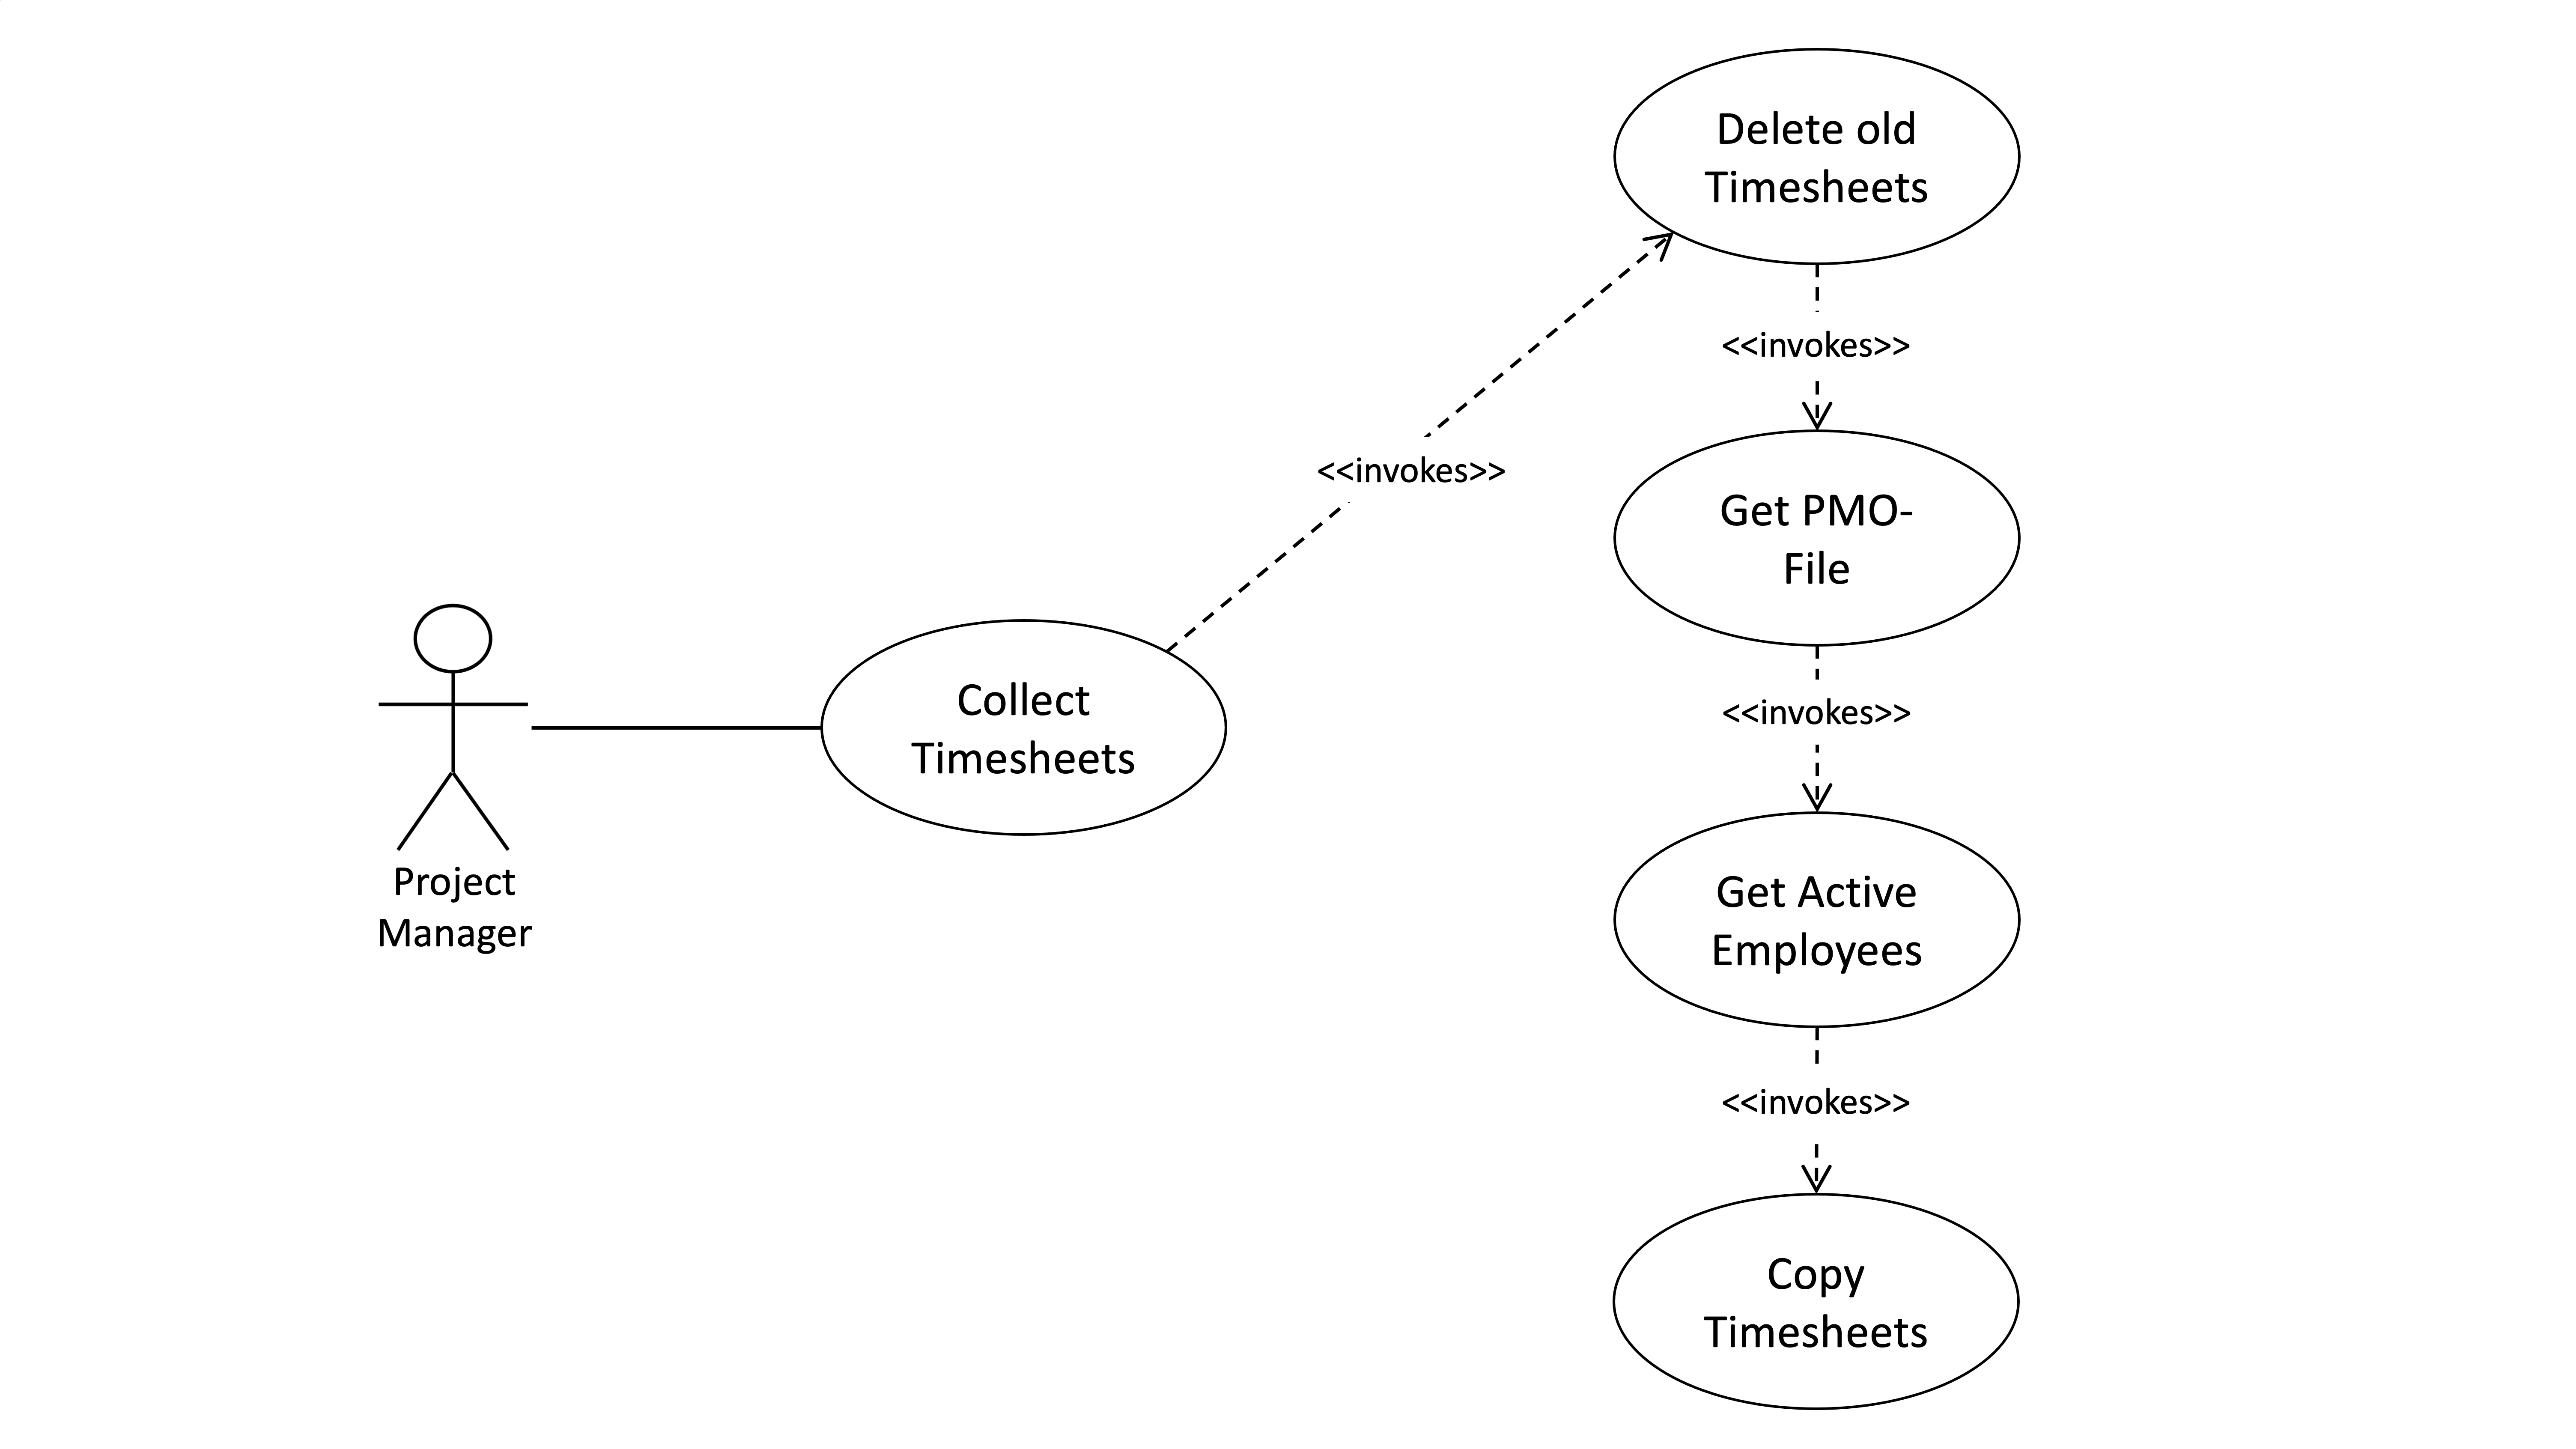
\includegraphics[width=\textwidth]{use-case-diagram.png}
    \caption{Use-Case Diagramm}
    \label{fig:use-case-diagram}
\end{figure}

\subsection{Akzeptanzkriterien}
Um die Implementierung als erfolgreich zu bewerten, müssen folgende Kriterien erfüllt sein:
\begin{itemize}
\item Die Parameter, wie zum Beispiel Projektname und vordefinierte Ordner IDs werden korrekt aus der Konfiguration gelesen und verwendet.
\item Alle Mitarbeiter, die im Projektmanagement-File den Status \glqq{aktiv}\grqq{} haben, werden korrekt ermittelt.
\item Die Timesheets für den zuvor definierten Monat werden für alle aktiven Mitarbeiter in das temporäre Verzeichnis kopiert.
\end{itemize}

\subsection{Testfälle}
Nachfolgende Testfälle wurden definiert, um die Implementierung zu testen:
\begin{itemize}
\item \textbf{Testfall 1:} Einlesen der Konfigurationsdatei und Einsammeln der Timesheets
\item \textbf{Testfall 2:} Einlesen der Konfigurationsdatei und Einsammeln der Timesheets mit Fehler
\end{itemize}

Für die Cloud-Migration der PMO-Tools war eine Umstrukturierung aufgrund der bestehenden Anwendungsstruktur notwendig. Dazu wurde die Anwendung umgeschrieben und in eine Springboot App umgewandelt. Alle Funktionen der ursprünglichen Anwendung mussten somit entsprechend in Java repliziert werden, der Aufwand dabei hängt stark von der Komplexität der jeweiligen Funktion ab. Desweiteren war es nötig, die Box-\ac{API} in die Anwendung zu integrieren, da die zuvor verwendete Zugriffsmethode nicht migrationsfähig gewesen wäre.